\subsection{Parameter estimation of speed distribution}
\label{section_speed_modeling}
In this section, we modeling the speed distribution.Because the probability will be influenced by the length of speed range, so we choose the cumulative distribution for modeling. Then we fit the cumulative distribution to get the cumulative probability distribution function, and then take a derivative with it to obtain the speed probability distribution.

Fig.\ref{formular_ccdf_speed} plots the cumulative distribution of speed. From the figure we can get following information:
\begin{itemize}
  \item In the speed range from about 0 to 40 km/h, the distributions show a linear relationship. While after the range, an exponential relationship can be observed.
  \item For vacant status, the distributions are similar. But on March.5 and 6, 2011, the curves show more similarity than on the other days.
  \item For vacant status, the speed distribution differs with each other evenly.
\end{itemize}

 A segmented function is chosen to fit the cumulative distributions and estimated the parameters. Especially, we respectively discuss the distribution for vacant status on workdays and weekend.
The fit formulas are given as formulas \ref{formular_ccdf_speed}.

\begin{equation}\label{formular_ccdf_speed}
\left\{
\begin{array}{ll}
 g(x)=a*x+b & x \in [0,40]\\
 f(x)=1-exp(-c*x-d)& x\in(40,120]\\
\end{array}
\right.
\end{equation}


Fig. \ref{figure_fit_ccdf_speed} also plots the fit results. For vacant status, we discuss the condition for that on workdays and weekend. The blue lines represent the fitting results for the speed range $[0,40] km/h$. And the red lines plot the fitting results for speed range $(40,180] km/h$.
We also fit the cumulative speed distribution for each status, shown as the right bottom in fig.\ref{figure_fit_ccdf_speed}.

\begin{figure}[htbp]
\centering
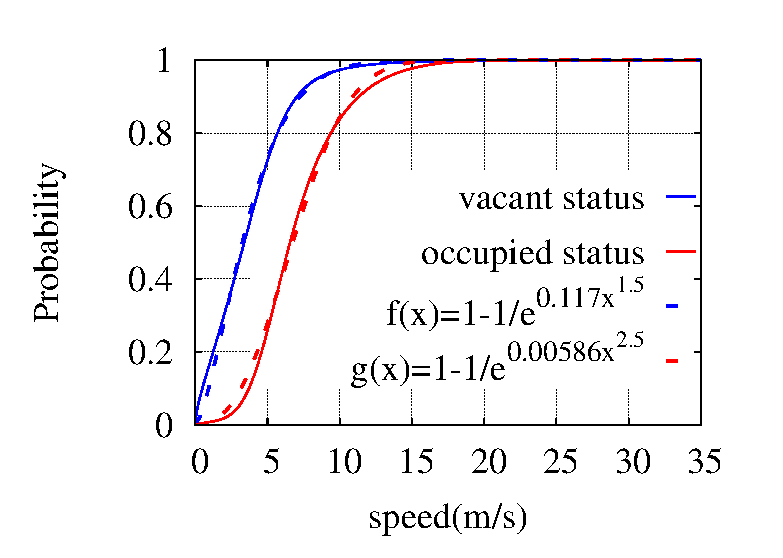
\includegraphics[width=0.4\textwidth]{figures_201103/fit/speedfit.eps}\\
\caption{The fit result of the cumulative speed distributions.}\label{figure_fit_ccdf_speed}
\end{figure}

The rms of residuals for each fit are as table \ref{table_rms}.The smaller rms of residuals means better fitting. In the table, the values are all less than 0.01, showing good similarity.

\begin{table}[!t]
\caption{The rms of residuals of fitting curves}\label{table_rms}
\centering
\begin{tabular}{l|c}
  \hline
  % after \\: \hline or \cline{col1-col2} \cline{col3-col4} ...
  Categories & rms of residuals  \\
  \hline
  $g_{status=0}^{workday}(x)$[0,40] & 0.00272264\\
  $g_{status=0}^{weekend}(x)$[0,40] & 0.00386982  \\
  $f_{status=0}(x)$(40,120] & 0.00148225\\
  $g(x)_{status=1}$[0,40]& 0.0176819 \\
  $f(x)_{status=1}$(40,120] & 0.00760913\\
  $g(x)_{status=0,1}$[0,40]& 0.0160319\\
  $f(x)_{status=0,1}$[40,120]& 0.00299414\\
  \hline
\end{tabular}
\end{table}

